\documentclass[10pt,a4paper]{article}
\usepackage[latin1]{inputenc}
\usepackage{amsmath}
\usepackage{amsfonts}
\usepackage{amssymb}
\usepackage{graphicx}
\usepackage{hyperref}
\usepackage{glossaries}
\usepackage{float}

\newcommand{\kx}{k_x}
\newcommand{\ky}{k_y}
\newcommand{\meff}{m_\text{eff}}

\newcommand{\img}{./images}
\loadglsentries{glossary.tex}
\makeglossaries
\begin{document}
\title{Progress}
\maketitle
%%%%%%%%%%%%%%%%%%%%%%%%%%%%%%%%%%%%%%%%%%%%%%%%%%%%%%%%%%%%%%%%%%%%%%%%%%%%%%%
\section{System description}
	\begin{figure}[H]
		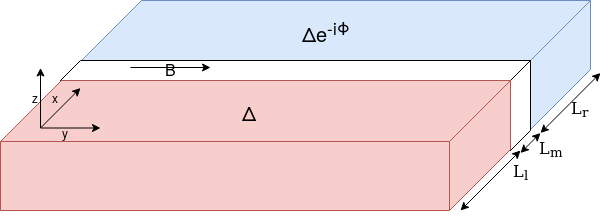
\includegraphics[width=\linewidth]{\img/system.png}
		\caption{System overview}
	\end{figure}
	
	\begin{align}
		H &= H_0(\tau_z \otimes \sigma_0) + 
		H_\text{Z} (\tau_0 \otimes \sigma_z) +
		(\tau_z \otimes H_\text{SO}) +
	 H_\text{SC}(\tau_y \otimes \sigma_0) \\
		H_0 &= \frac{\hbar^2}{2\meff}\left(\kx^2 + \ky^2\right) - \mu \\
		H_\text{Z} &= g \mu_B B  \left(\Theta(-x) - \Theta(L_m-x)\right)  \\
		H_\text{SO} &= \alpha \left( \ky \sigma_x - \kx \sigma_y \right)\\
		H_\text{SC} &= \Delta \exp \left(i \theta \Theta(x-L_m) \right)
	\end{align}
	Where: 
	\begin{equation}
	\Theta(x) = 
	\begin{cases}
	1,& x>0\\
	0,& \text{otherwise}
	\end{cases}
	\end{equation}
	\subsection{Assumptions and limitations of model}
%		[TODO: LIST ASSUMPTIONS AND LIMITATIONS: SPIN ORBIT DRESSELHAUS, SC MODEL, ETC.]
	\subsection{System parameters}
	\begin{table}
		\begin{tabular}{|c|c|c|c|}
			\hline 
			Variable & Description & Typical value & Default value \\ 
			\hline 
			$g_\text{factor}$ & Magnetic g-factor of material & ~10 & 10 \\ 
			\hline 
			$\mu$ & Chemical potential &  10 - 30 meV & 1 meV\\ 
			\hline 
			$\alpha$ & Spin orbit coupling strength &  30 meV nm & 30 meV nm \\ 
			\hline 
			$\Delta$ & Superconducting gap & 0.2 - 0.3 meV & 0.18 meV\\ 
			\hline 
			$B$ & In-plane magnetic field strength along stripe direction(y) & 0 - 1 T & 0.2 T \\ 
			\hline 
			$\phi$ & Relative phase between superconductors &  0 - 2$\pi$ & $\pi$\\ 
			\hline 
			$\text{L}_\text{l}$ & Width of left superconductor & $\infty$ & 500 nm \\
			\hline 
			$\text{L}_\text{m}$ & Width of right superconductor & $\infty$ & 500 nm \\
			\hline
			$\text{L}_\text{r}$ & Width of middle "normal" strip & 100 - 1000 nm & 250 nm \\
			\hline
			$\text{L}_\text{y}$ & Length of system & \textgreater1000 nm & 4000 nm\\
			\hline
			$T$ & Temperature of system & 0.25 - 1.2K & 0 K\\
			\hline
		\end{tabular} 
	\caption{Description of system parameters, along with typical valuses, as well as a default value which is the used value when no other value has been specified.}
	\label{tbl:system_pars}
	\end{table}
	Describe parameters provided by experimentalists(electron density 3e15-3e16, effective mass 0.04me)
%%%%%%%%%%%%%%%%%%%%%%%%%%%%%%%%%%%%%%%%%%%%%%%%%%%%%%%%%%%%%%%%%%%%%%%%%%%%%%%
\section{Parametric overview of the system}
%------------------%
	\subsection{Important metrics}
	We study the influence of the different parameters on the physics of the system by considering a handful of metrics. We list them below, along with how they are computed and what their physical significance is.
		\begin{itemize}
			\item \Gls{Ethouless}
				\begin{align}\label{eq:thouless}
				E_\text{Th} = TN\delta
				, && \delta = \frac{\hbar^2 \pi^2}
				{2 m_e \left( 2 L_m \right)^2}
				\end{align}
			Where $T$ is the transparancy of the junction, and N the number of bands.
			\item Topological invariant: Pfaffian sign
				\subitem The system is extended to infinity and the Pfaffian allows us compute the parity of number of states with positive energy of the system, disregarding the holes. If the resulting topological invariant is -1, we can conclude that if the system were to be made finite, it could potentially support majorana bound states.

			\item Topological energy gap
				\subitem The system is again extended to infinity, and the energy difference between the majorana bound states(energy 0) and the next lowest lying band is calculated, using the bisection method.
				
			\item (critical) current, phase offset in current-phase relationship
				\subitem The system is extended to infinity, and the current density is calculated at a cut in the non-superconducting section.
			
			\item Junction transparency
				\subitem The transparency is using kwant. It gives an indication of 
		\end{itemize}
%------------------%
\newpage
	\subsection{Varying magnetic field strength and superconducting phase}
		In this section, we vary the Zeeman field strength and superconducting phase, calculating the topological invariant. 
		From the Pientka paper, we would expect diamond like structures to appear along the magnetic field axis, spaced apart with a distance equal to the Thouless energy. We indeed find this to be the case(figure \ref{fig:lmZPpfaf}). By varying the width of the middle strip we adjust the Thouless energy, and we see clearly find the diamonds shaped apart by the Thouless energy.
		
		Beyond a certain Zeeman field, we see(although not shown in the figure) that the diamond pattern ceases and turns into stripes independent of phase. At this point, the magnetic field is so strong that bands cross, and our model becomes unphysical. Applying a magnetic field in the superconducting leads as well, lowers the field where this happens.
		
		We will use this phase-Zeeman plot throughout the report as both parameters are easily tunable whem compared to the rest, and the diamond structure gives us an analysable feature.
		
		\subsubsection{Anna\&Bas}
		Independence of phase should indeed appear beyond a certain magnetic field, when normal reflection becomes very big. When Zeeman is turned on in leads, in a system with infinite sc leads($L_l, L_r \rightarrow \infty$), only a single half diamond appears.
		
	\begin{figure}[H]
		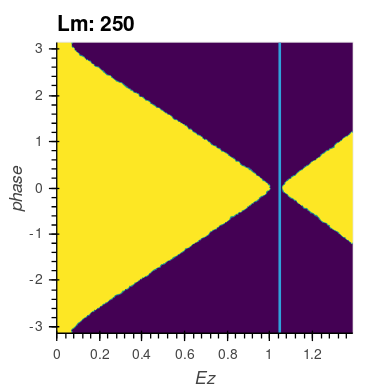
\includegraphics[width=0.5\textwidth]{\img/lmZPpfaf/pB250.png}
		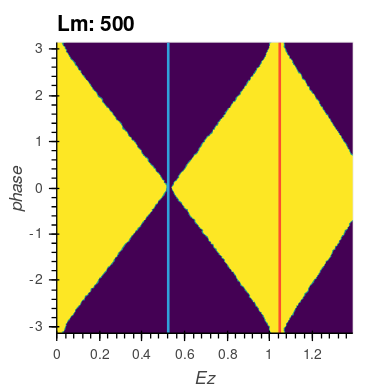
\includegraphics[width=0.5\textwidth]{\img/lmZPpfaf/pB500.png}
		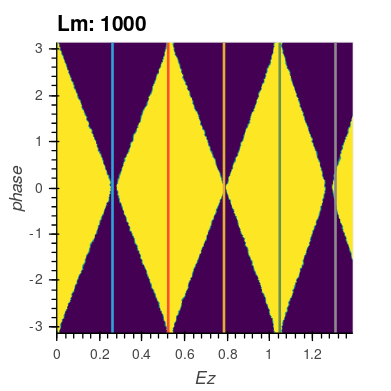
\includegraphics[width=0.5\textwidth]{\img/lmZPpfaf/pB1000.png}
		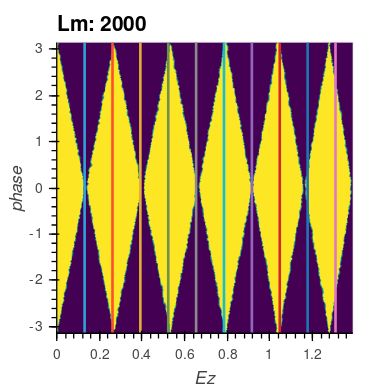
\includegraphics[width=0.5\textwidth]{\img/lmZPpfaf/pB2000.png}
		\caption{Topological regime(blue is topological) vs superconducting phase and magnetic field strength, for different strip widths. The lines indicate integer multiples of the Thouless energy, see table \ref{table:thouless}}
		\label{fig:lmZPpfaf}
	\end{figure}

	%------------------%
	\subsection{Varying system dimensions}
	 As mentioned before, widening the junction lowers the Thouless energy, which makes the topological regime accesible at lower magnetic fields. We are however also interested in how big the resulting topological gap is. 
	 
	 In figure \ref{fig:lmZPgap}, we plot the energy gap around zero energy. We see that increasing the middle strip width has the effect of lowering the gap in the topological region. The system we are considering is considered an intermediate to long junction: $E_\text{Th} \gtrapprox \Delta$ or $E_\text{Th} \gg \Delta$. This implies that the relation between the induced gap and the Thouless energy and superconducting gap is $\Delta_\text{ind} \propto E_\text{Th}$[VUIK]. It would be interesting to investigate wether the gap indeed varies proportionally to the Thouless energy.
	 
	 We see that width of the gapless strips along the topological borders are quite wide, requiring very high magnetic field to reach a gapped topological state of the system.
 	\subsubsection{Anna\&Bas}
 	Relation between topological gap and thouless is given in the paper. Investigate what regime we are in(short, long intermediate junction). Higher chemical potential would also be a thing
	\begin{table}[H]
		\centering
		\begin{tabular}{|c|c|}
			\hline 
			$L_\text{m} (nm)$ & $E_\text{Th} (meV)$ \\ 
			\hline 
			250 & 1.05 \\ 
			\hline 
			500 & 0.523 \\ 
			\hline 
			1000 & .262 \\ 
			\hline 
			5000 & .0523 \\ 
			\hline 
		\end{tabular} 
		\caption{Thouless energy for different system widths calculated using \ref{eq:thouless}, asssuming unit transparency.}
		\label{table:thouless}
	\end{table}
	
	
	\begin{figure}[H]
		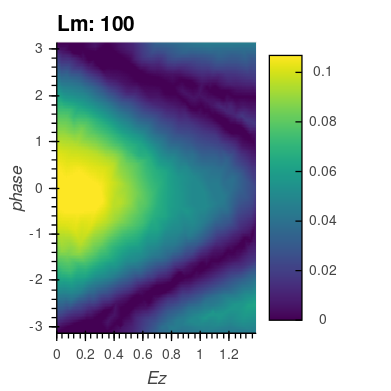
\includegraphics[width=0.5\textwidth]{\img/lmgap/lm100.png}
		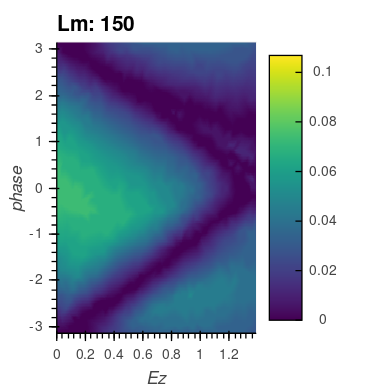
\includegraphics[width=0.5\textwidth]{\img/lmgap/lm150.png}
		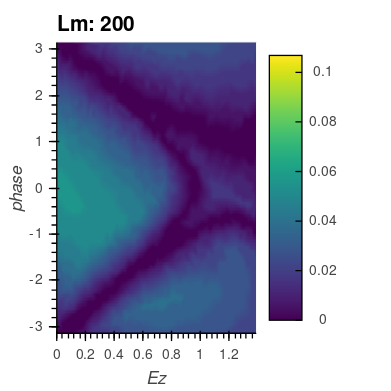
\includegraphics[width=0.5\textwidth]{\img/lmgap/lm200.png}
		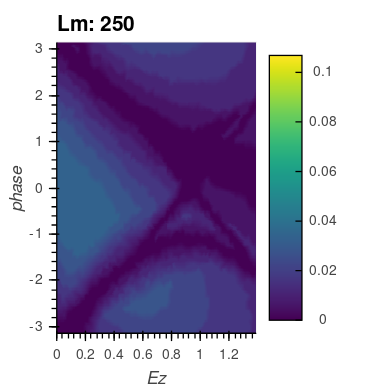
\includegraphics[width=0.5\textwidth]{\img/lmgap/lm250.png}
		%				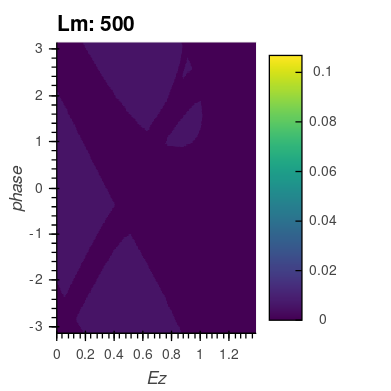
\includegraphics[width=0.24\textwidth]{\img/lmgap/lm500.png}
		\caption{Energy gap vs superconducting phase and magnetic field strength, for different strip widths.}
		\label{fig:lmZPgap}
	\end{figure}
%------------------%	
\newpage	
	\subsection{Varying chemical potential and magnetic field strength}
		We vary the chemical potential and zeeman field plotting both the topology as well as the energy gap of the system. We do this for two situations; with and without zeeman field in the leads. 
		
		In figure \ref{fig:muZ_zinsc}, we consider the system with zeeman field in the superconducting part. We see a chainlike structures as described in the Pientka paper. The first chain opens up as a function of phase, and forms a large strip where the system is topological for a wide range of chemical potential. We see from the energy gap plots that only the first 'chain' has is gapless.
		
		In figure \ref{fig:muZnosc}, we plot the system without magnetic field in the leads. With respect to the system with zeeman in the leads, it almost seems like the plot has undergone rescaling. The other diamond chains are not visible in this plot, and only appear when we greatly adjust the axes(not shown). We also see that although we can clearly see the gap closing bands(topological borders) in the gap plots, the underlying gap size does not seem greatly affected by being in topological region or not.
	\subsubsection{Anna\&Bas}
	Experiment was run at very small chemical potential, which could cause you to see discretization of the leads. It also matters whether the system is 2d infinite or not. The diamond chains are caused by gap closings of the different bands. If the system is 2d infinite, the gap is always closed.
	
			\begin{figure}[H]
			\begin{tabular}{cc}
				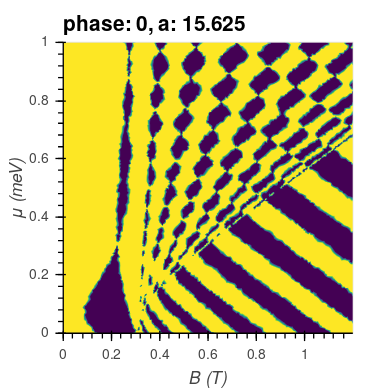
\includegraphics[width=0.35\textwidth]{\img/pfafmuZ_zinsc/muB0.png}&
				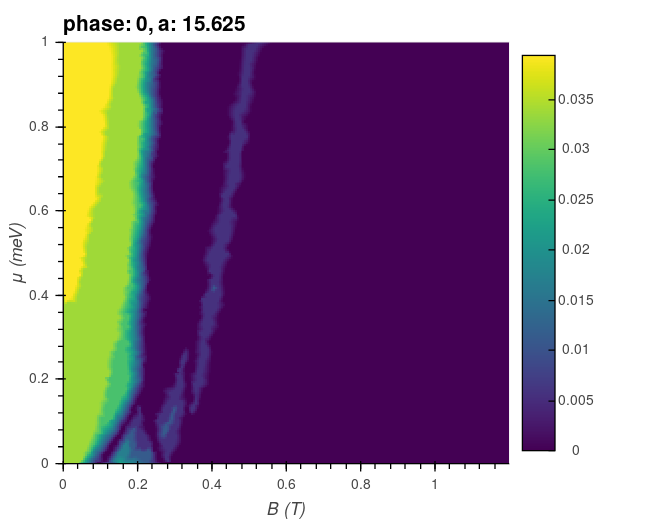
\includegraphics[width=0.45\textwidth]{\img/gapmuZ_zinsc/00_gap_muZ.png}\\
				&
				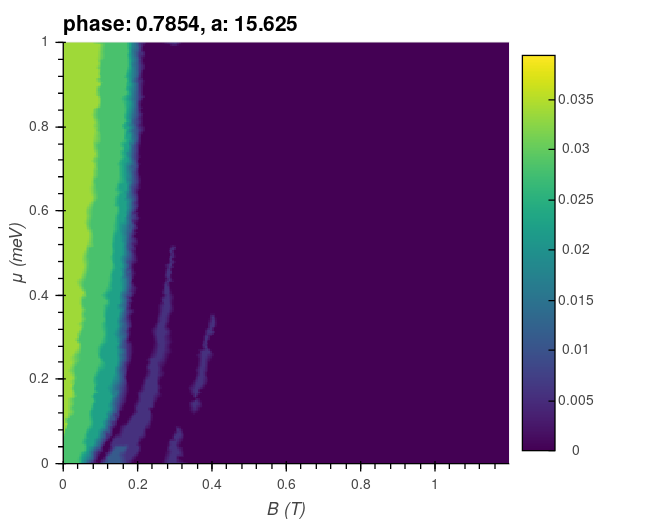
\includegraphics[width=0.45\textwidth]{\img/gapmuZ_zinsc/25_gap_muZ.png}\\
				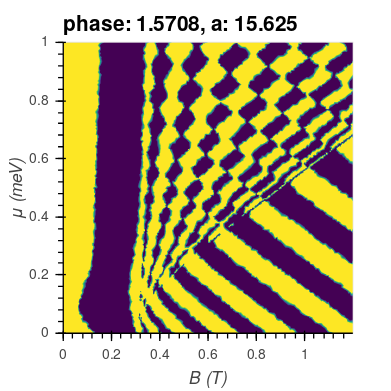
\includegraphics[width=0.35\textwidth]{\img/pfafmuZ_zinsc/muB5.png}&
				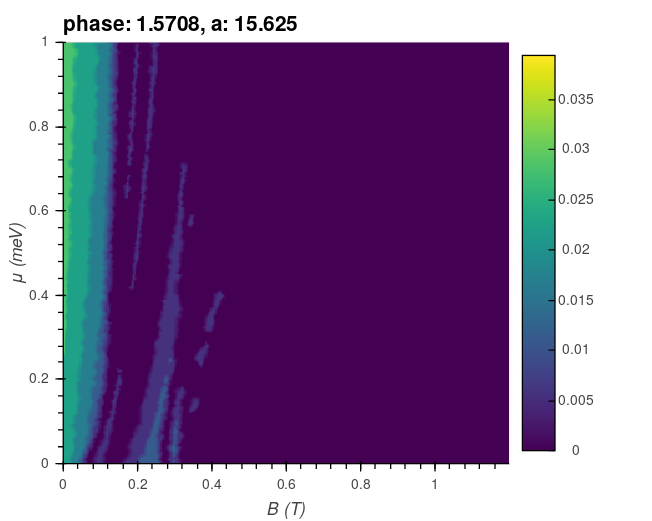
\includegraphics[width=0.45\textwidth]{\img/gapmuZ_zinsc/50_gap_muZ.png}\\
				&
				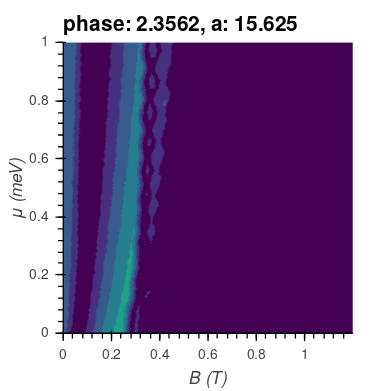
\includegraphics[width=0.45\textwidth]{\img/gapmuZ_zinsc/75_gap_muZ.png}\\
				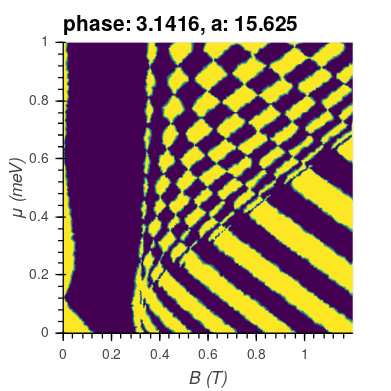
\includegraphics[width=0.35\textwidth]{\img/pfafmuZ_zinsc/muB1.png}&
				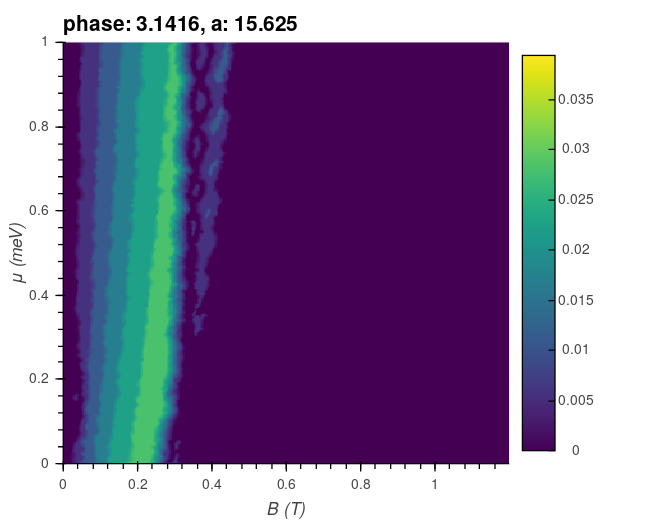
\includegraphics[width=0.45\textwidth]{\img/gapmuZ_zinsc/1_gap_muZ.png}\\
			\end{tabular}
		\caption{Topological regime(blue is topological) and energy gap vs chemical potential and magnetic field strength, assuming zeeman field persists in the superconductor}\label{fig:muZ_zinsc}
			\end{figure}


\begin{figure}[H]
	\begin{tabular}{cc}
				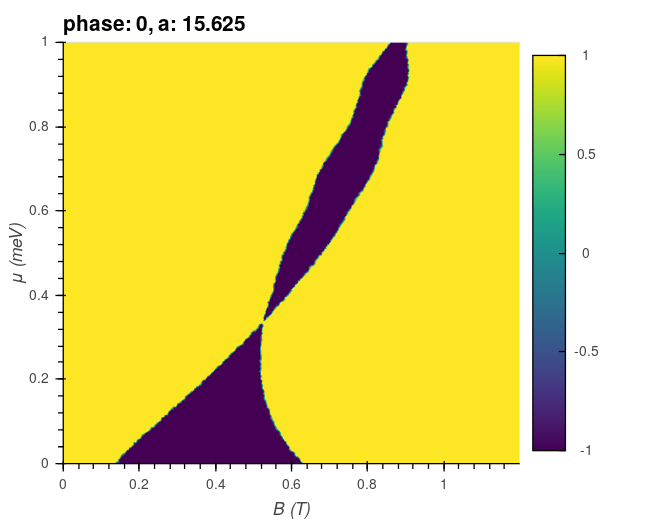
\includegraphics[width=0.4\textwidth]{\img/pfafmuZ_noZinsc/00pfafmuZnoZinSC.png}&
			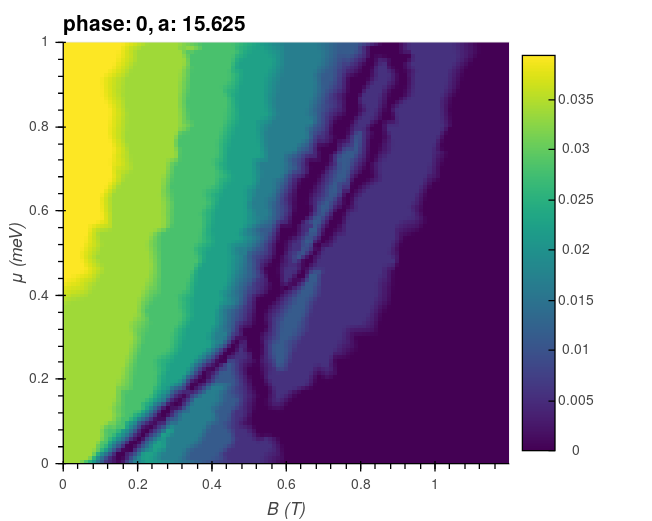
\includegraphics[width=0.4\textwidth]{\img/gapmuZ_noZinsc/0gapmuZ.png}\\
				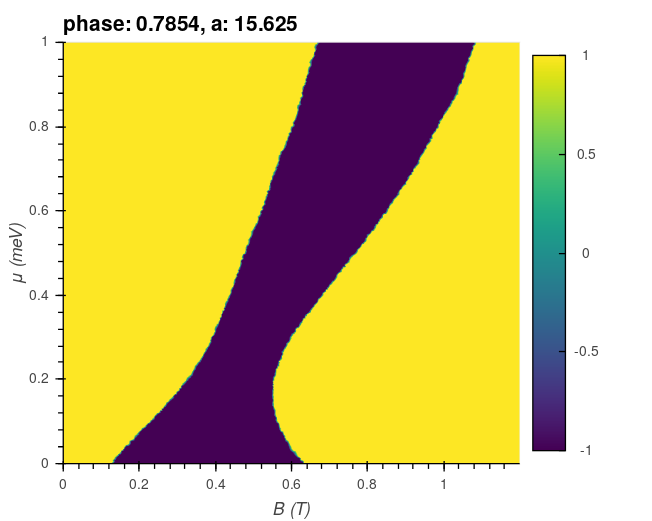
\includegraphics[width=0.4\textwidth]{\img/pfafmuZ_noZinsc/25pfafmuZnoZinSC.png}&
			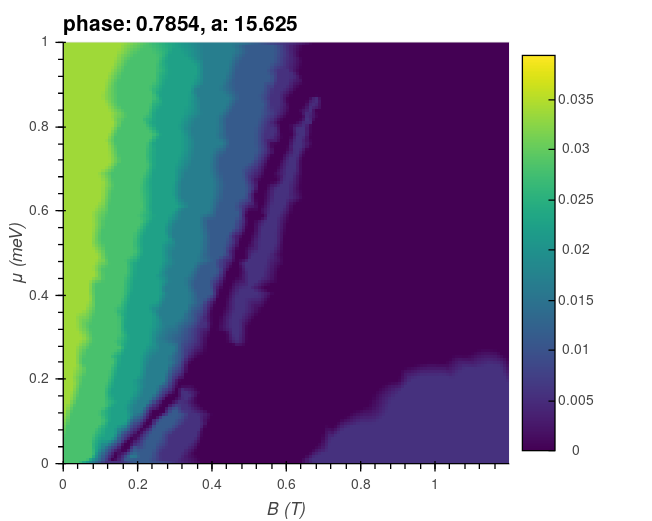
\includegraphics[width=0.4\textwidth]{\img/gapmuZ_noZinsc/25gapmuZ.png}\\
				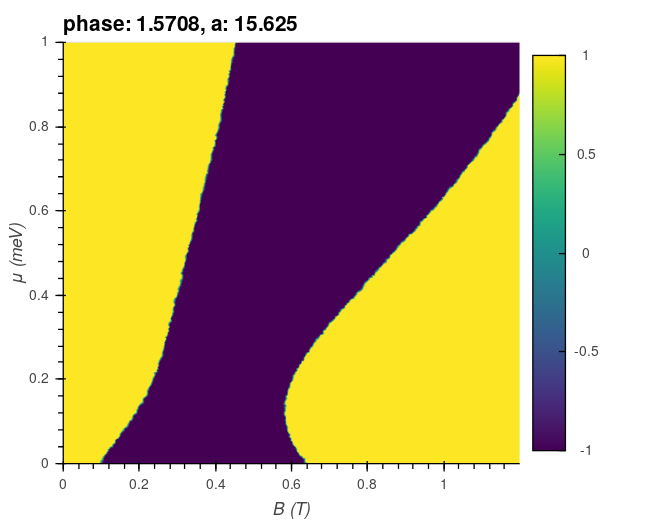
\includegraphics[width=0.4\textwidth]{\img/pfafmuZ_noZinsc/50pfafmuZnoZinSC.png}&
			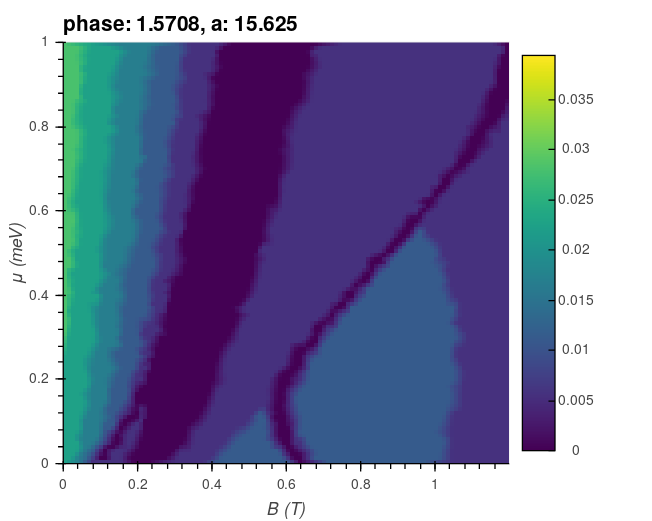
\includegraphics[width=0.4\textwidth]{\img/gapmuZ_noZinsc/50gapmuZ.png}\\
				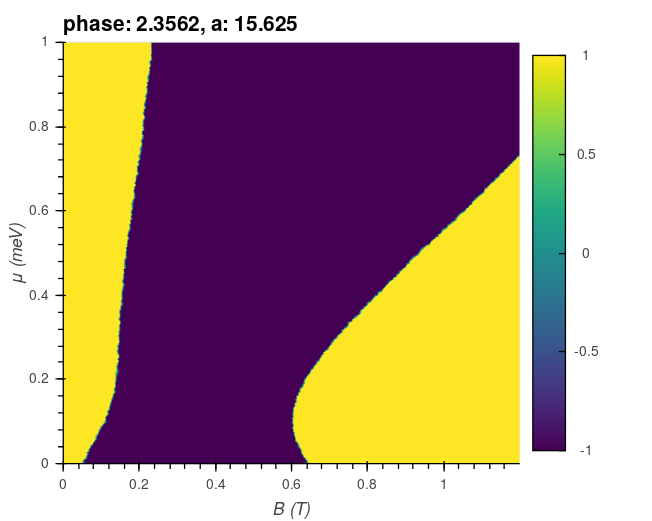
\includegraphics[width=0.4\textwidth]{\img/pfafmuZ_noZinsc/75pfafmuZnoZinSC.png}&
			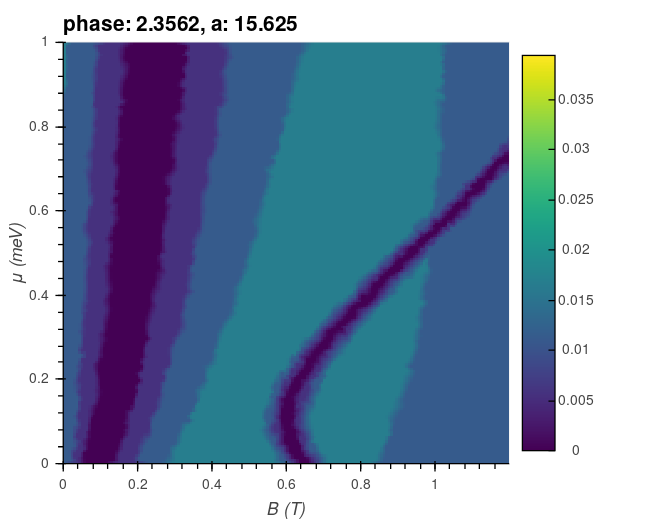
\includegraphics[width=0.4\textwidth]{\img/gapmuZ_noZinsc/75gapmuZ.png}\\
				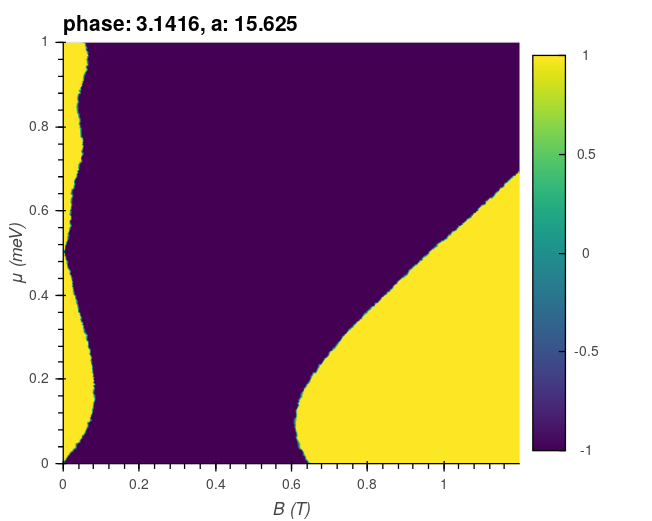
\includegraphics[width=0.4\textwidth]{\img/pfafmuZ_noZinsc/1pfafmuZnoZinSC.png}&
			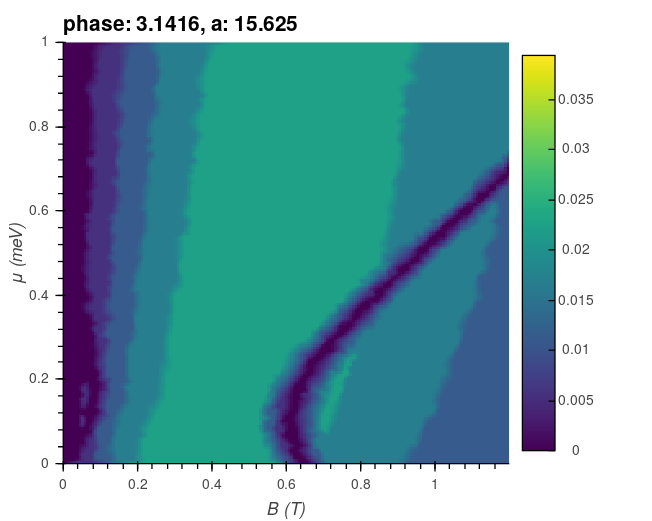
\includegraphics[width=0.4\textwidth]{\img/gapmuZ_noZinsc/1gapmuZ.png}\\
	\end{tabular}\label{fig:muZnosc}
		\caption{Topological invariant and energy gap vs chemical potential and magnetic field strength, assuming zeeman field persists in the superconductor}
\end{figure}

%------------------%
\newpage
	\subsection{Varying spin-orbit}
	In figure \ref{fig:pfaf_pB_soi} and \ref{fig:gap_pB_soi} we plot topology and energy gap respectively as a function of phase and magnetic field, for different values of the spin orbit coupling. From the topology, wee see that variation of SOI influences both the shape of the diamonds as well as offsets their position. From the Pientka paper, we know that both are also symptoms of non unit junction transparency. It would be interesting to indeed investigate this.
	
	The influence of varying spin orbit coupling seems to be limited. Although at lower spin orbit couplings, we see strands of gap-closings, which would be interesting to investigate, the energy gap in the topological region does not vary much.		\subsubsection{Anna\&Bas}
	Effects seen could be due to not counting chemical potential from the bottom of the band, accounting for the term $\propto m\alpha^2$. Check ifthis is indeed the case. Check if this is indeed the case. 
	
	The gap closing might be due to BD1 symmetry. Note that the phase diagram there is $4\pi$ symmetric. Shifting phase by $\pi$ causes overall gauge of -1. Change gap on left and right lead to break symmetry, see if gap closings persist.
	
		\begin{figure}[H]
			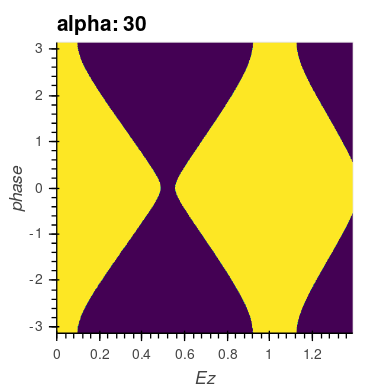
\includegraphics[width=0.192\textwidth]{\img/spinorbitZP/a30.png}
			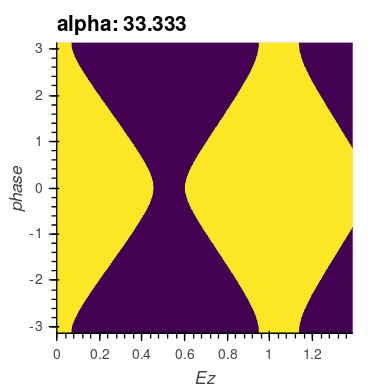
\includegraphics[width=0.192\textwidth]{\img/spinorbitZP/a33.png}
			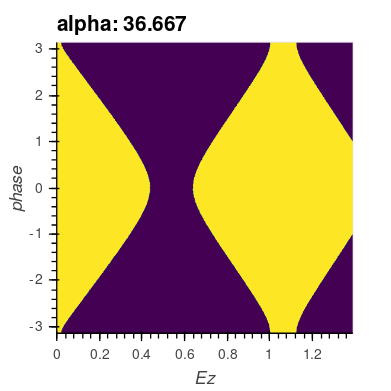
\includegraphics[width=0.192\textwidth]{\img/spinorbitZP/a36.png}
			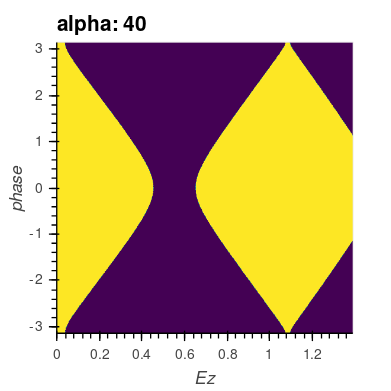
\includegraphics[width=0.192\textwidth]{\img/spinorbitZP/a40.png}
			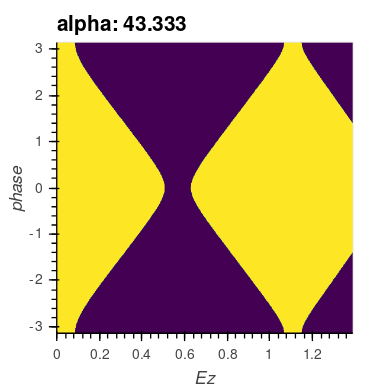
\includegraphics[width=0.192\textwidth]{\img/spinorbitZP/a43.png}
			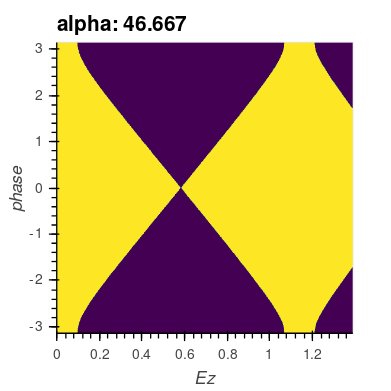
\includegraphics[width=0.192\textwidth]{\img/spinorbitZP/a46.png}
			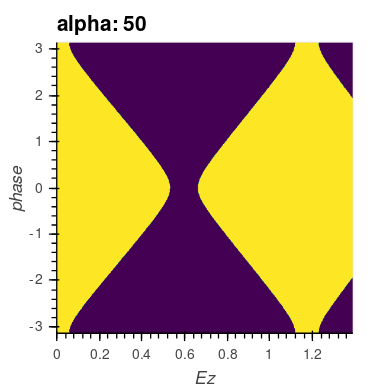
\includegraphics[width=0.192\textwidth]{\img/spinorbitZP/a50.png}
			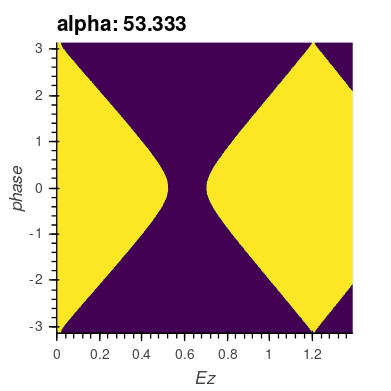
\includegraphics[width=0.192\textwidth]{\img/spinorbitZP/a53.png}
			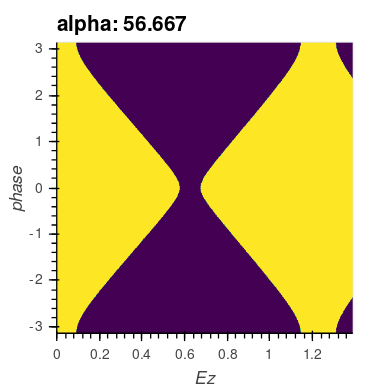
\includegraphics[width=0.192\textwidth]{\img/spinorbitZP/a56.png}
			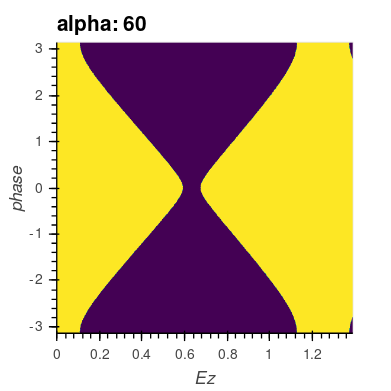
\includegraphics[width=0.192\textwidth]{\img/spinorbitZP/a60.png}
			\caption{Phase zeeman topology plot with increasing spin orbit. $L_\text{m}=500$nm}
			\label{fig:pfaf_pB_soi}
		\end{figure}
	
		\begin{figure}[H]
			\begin{tabular}{ccc}
				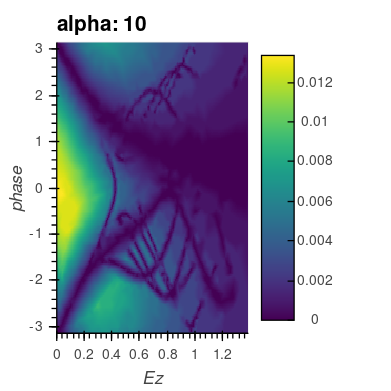
\includegraphics[width=0.33\textwidth]{\img/spinorbitGap/gap_pB_alpha10.png}&
				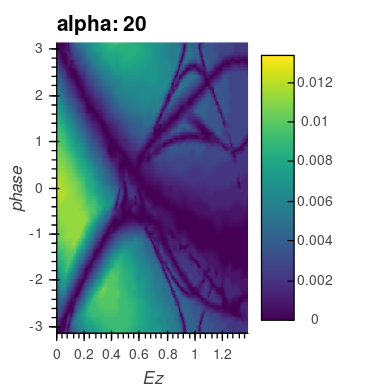
\includegraphics[width=0.33\textwidth]{\img/spinorbitGap/gap_pB_alpha20.png}&
				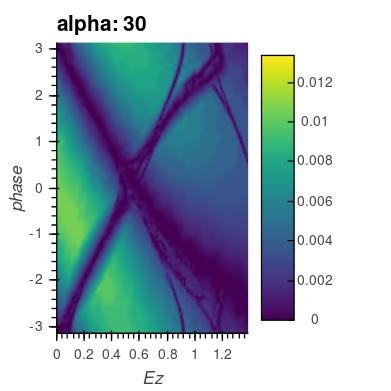
\includegraphics[width=0.33\textwidth]{\img/spinorbitGap/gap_pB_alpha30.png}\\
				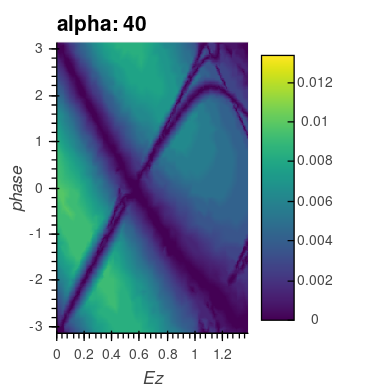
\includegraphics[width=0.33\textwidth]{\img/spinorbitGap/gap_pB_alpha40.png}&
				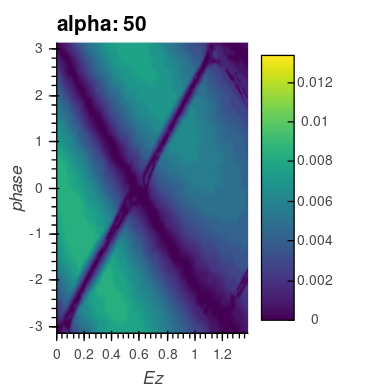
\includegraphics[width=0.33\textwidth]{\img/spinorbitGap/gap_pB_alpha50.png}&
				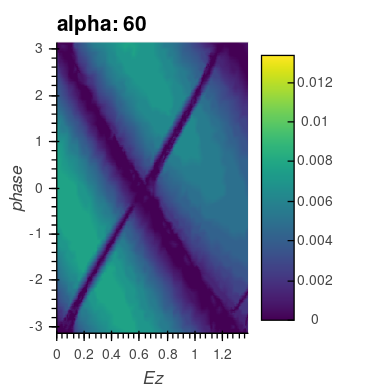
\includegraphics[width=0.33\textwidth]{\img/spinorbitGap/gap_pB_alpha60.png}\\
			\end{tabular}
			\caption{Phase zeeman energy gap plot with increasing spin orbit. $L_\text{m}=500$nm}
			\label{fig:gap_pB_soi}
		\end{figure}
%------------------%
\newpage	
	\subsection{Varying superconducting gap}
	Increasing the superconducting gap has the effect of reducing the energy gap somewhat. We also again see the appearance of gapless bands through the regions.
	
	\subsubsection{Anna\&Bas}
	Increase width of leads, and rerun experiments. It is weird that gap would decrease as $\Delta$ is increased. Look at band structure.
		\begin{figure}[H]
			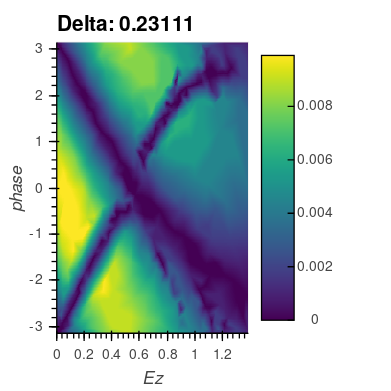
\includegraphics[width=0.24\textwidth]{\img/deltagapZPcurrent/d02.png}
			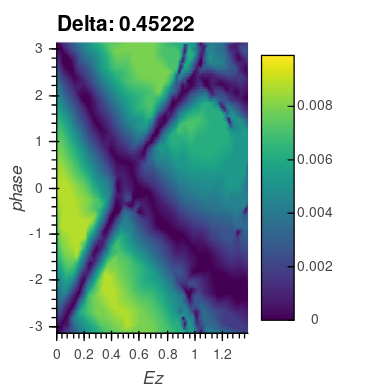
\includegraphics[width=0.24\textwidth]{\img/deltagapZPcurrent/d045.png}
			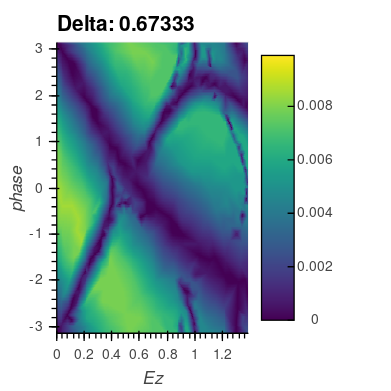
\includegraphics[width=0.24\textwidth]{\img/deltagapZPcurrent/d067.png}
			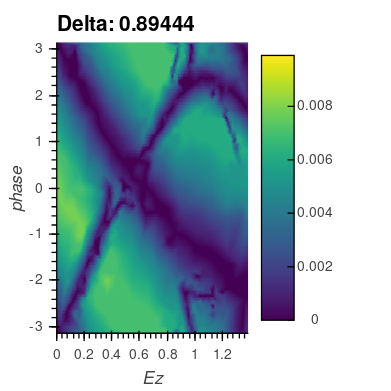
\includegraphics[width=0.24\textwidth]{\img/deltagapZPcurrent/d089.png}
			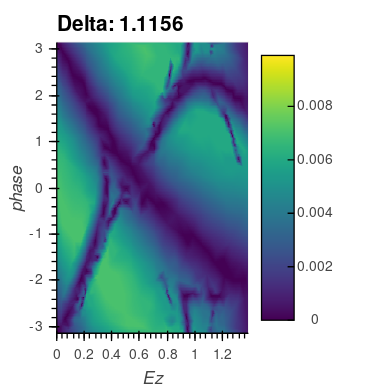
\includegraphics[width=0.24\textwidth]{\img/deltagapZPcurrent/d11.png}
			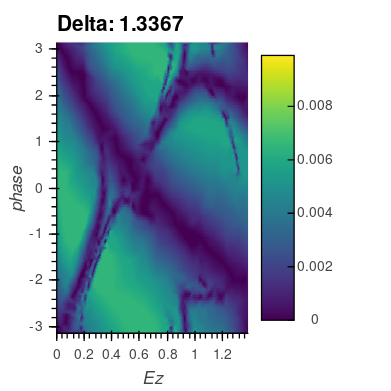
\includegraphics[width=0.24\textwidth]{\img/deltagapZPcurrent/d133.png}
			\includegraphics[width=0.24\textwidth]{\img/deltagapZPcurrent/d155.png}
			\includegraphics[width=0.24\textwidth]{\img/deltagapZPcurrent/d178.png}
			\includegraphics[width=0.24\textwidth]{\img/deltagapZPcurrent/d200.png}
			\caption{Phase zeeman plot with increasing spin orbit}
		\end{figure}
%------------------%	
\newpage
	\subsection{Varying temperature}
	\subsubsection{Anna\&Bas}
	It is normal to see non block wave phase minimizing current. The current can be split into two contributions. 
	Due to spin orbit coupling, in 2d infinite system, we have two circular fermi surfaces. The values for $\kx,\ky$ which lie on both fermi surfaces, are responsible for the block wave pattern. The region outside of that is responsible for a more sinosoidal pattern.
	So for low spin orbit coupling, the radii are almost the same, and it is all block wave.
		\begin{figure}[H]
			\begin{tabular}{rcc}
				a, T=0.025K&\includegraphics[width=0.4\textwidth]{\img/current/critcurr_lm200_T0025.png}&
				\includegraphics[width=0.4\textwidth]{\img/current/curr_lm200_T0025.png}\\
				\hline
				b, T=0.2K&\includegraphics[width=0.4\textwidth]{\img/current/critcurr_lm200_T02.png}&
				\includegraphics[width=0.4\textwidth]{\img/current/curr_lm200_T02.png}\\
				\hline
				c, T=0.6K&\includegraphics[width=0.4\textwidth]{\img/current/critcurr_lm200_T06.png}&
				\includegraphics[width=0.4\textwidth]{\img/current/curr_lm200_T06.png}\\
				\hline
			\end{tabular}
			\caption{Critical current(maximum minus minimum current) and current versus phase and magnetic field strength, assuming zeeman field does not persists in the superconductor. Width of normal strip is 200nm. Temperatures of a, b and c respectively: 0.025 K, 0.2K, 0.6K}
		\end{figure}
	
		\begin{figure}[H]
			\begin{tabular}{rcc}
				a, T=0.025K&\includegraphics[width=0.4\textwidth]{\img/current/critcurr_lm250_T0025.png}&
				\includegraphics[width=0.4\textwidth]{\img/current/curr_lm250_T0025.png}\\
				\hline
				b, T=0.2K&\includegraphics[width=0.4\textwidth]{\img/current/critcurr_lm250_T02.png}&
				\includegraphics[width=0.4\textwidth]{\img/current/curr_lm250_T02.png}\\
				\hline
				c, T=0.6K&\includegraphics[width=0.4\textwidth]{\img/current/critcurr_lm250_T06.png}&
				\includegraphics[width=0.4\textwidth]{\img/current/curr_lm250_T06.png}\\
				\hline
			\end{tabular}
			\caption{Critical current(maximum minus minimum current) and current versus phase and magnetic field strength, assuming zeeman field does not persists in the superconductor. Width of normal strip is 250nm. Temperatures of a, b and c respectively: 0.025 K, 0.2K, 0.6K}
		\end{figure}
%%%%%%%%%%%%%%%%%%%%%%%%%%%%%%%%%%%%%%%%%%%%%%%%%%%%%%%%%%%%%%%%%%%%%%%%%%%%%%%
\clearpage
\printglossaries
\end{document}

